\documentclass[onecolumn,draftclsnofoot, 10pt, compsoc]{IEEEtran}

\usepackage{graphicx}
\usepackage[section]{placeins}
\usepackage{caption}

\usepackage{amssymb}                                         
\usepackage{amsmath}                                         
\usepackage{amsthm}                                

\usepackage{alltt}                                           
\usepackage{float}
\usepackage{color}
\usepackage{url}

\usepackage{balance}
\usepackage[TABBOTCAP, tight]{subfigure}
\usepackage{enumitem}
\usepackage{pstricks, pst-node}
\usepackage{url}
\usepackage{setspace}

\usepackage{etoolbox}
\AtBeginEnvironment{quote}{\singlespacing\vspace{-\topsep}\small}

%\input{pygments.tex}

\usepackage{geometry}
\geometry{left=0.75in,right=0.75in,top=0.75in,bottom=0.75in}
\parindent = 0.0 in
\parskip = 0.1 in


\def \ParSpace{\vspace{.75em}}
\def \Jeremy{			Jeremy Fischer}
\def \Class{		Parallel Programming}
\def \Assn{		Project 7: OpenCL / OpenGL Particle System}
\def \School{	Oregon State University}
\def \Professor{		Matthew Meyn}

\newcommand{\cred}[1]{{\color{red}#1}}
\newcommand{\cblue}[1]{{\color{blue}#1}}

\newcommand{\NameSigPair}[1]{
		\par
		\makebox[2.75in][r]{#1} \hfil 	\makebox[3.25in]{\makebox[2.25in]{\hrulefill} \hfill			
		\makebox[.75in]{\hrulefill}}
		\par\vspace{-12pt} \textit{
			\tiny\noindent
			\makebox[2.75in]{} \hfil		
			\makebox[3.25in]{
				\makebox[2.25in][r]{Signature} \hfill	\makebox[.75in][r]{Date}
			}
		}
}










%%%%%%%%%%%%%%%%%%%%%%%%%%%%%%%%%%%%%%%
\begin{document}
\begin{titlepage}
    \pagenumbering{gobble}
    \begin{singlespace}
    	
\includegraphics[height=4cm]{coe.eps}
        \hfill  
        \par\vspace{.2in}
        \centering
        \scshape{
            \vspace{.5in}
            \textbf{\Large\Assn}\par
            \textbf{\large\Class}\par
            \large{
            	\today \\Spring Term
        	}
            \vfill
            {\large Prepared for}\par
            \huge \School\par
            \vspace{5pt}
            {\Large{\Professor}\par}
            {\large Prepared by }\par

            \vspace{5pt}
            {\Large
                {\Jeremy}\par
            }
            \vspace{20pt}
        }

    \end{singlespace}
\end{titlepage}
\newpage
\pagenumbering{arabic}

% 7. uncomment this (if applicable). Consider adding a page break.
%\listoffigures
%\listoftables
\clearpage



\section{What machine you ran this on?}
	I ran this test on a 2015 Macbook Pro, 2.2 GHz Intel Core i7, 16 GB 1600 MHz DDR3 using Xcode.

		



\section{What dynamic thing did you do with the particle colors}
	I added two spheres, a green and a blue, and started the pixels directly between the two. The particles then explode outwards and morph into the color of the sphere that particle first collided with.



\section{Include at least one screen capture image of your project in action}
	
	\begin{figure}[H]
		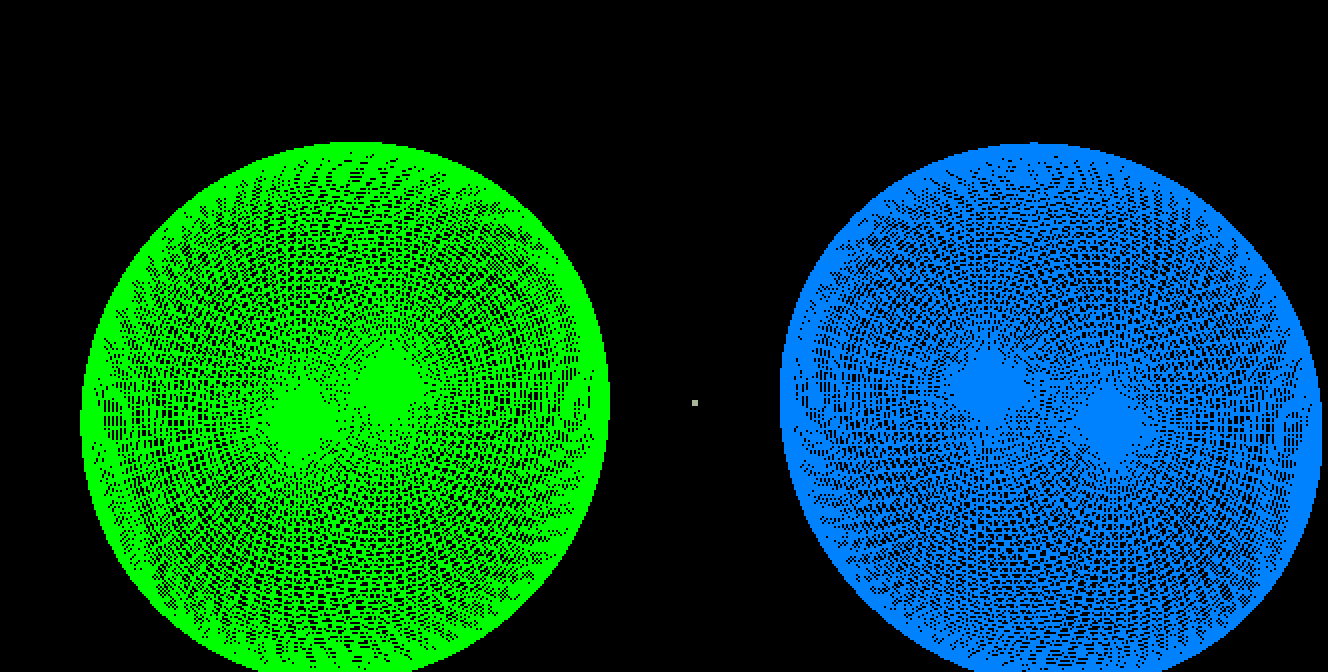
\includegraphics[width=14cm]{pic1}
		\caption{Phase 1}
	\end{figure}
	\begin{figure}[H]
		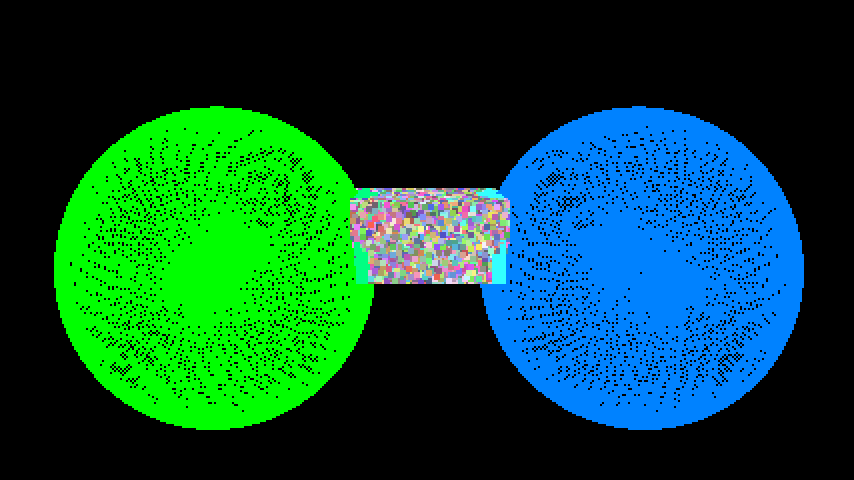
\includegraphics[width=14cm]{pic2}
		\caption{Phase 2}
	\end{figure}

	\begin{figure}[H]
		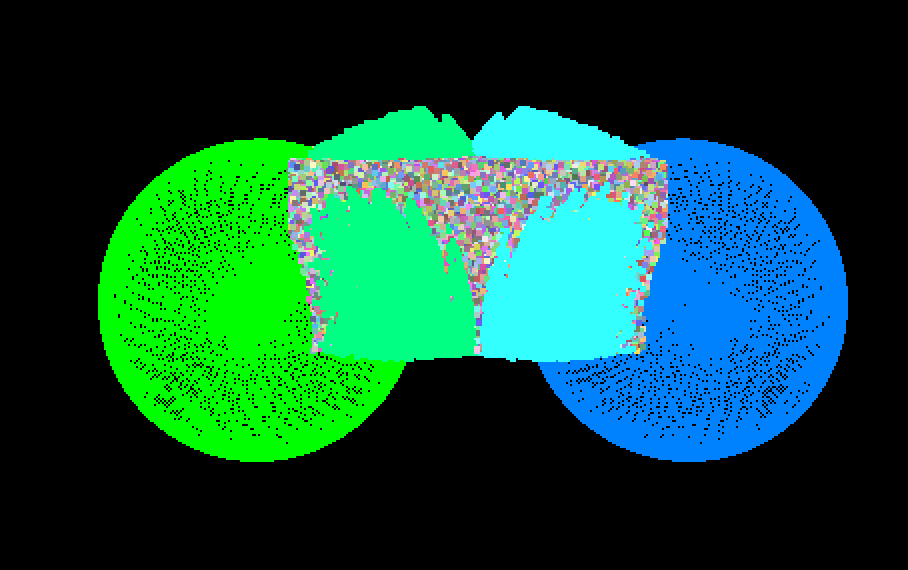
\includegraphics[width=14cm]{pic3}
		\caption{Phase 3}
	\end{figure}
	\begin{figure}[H]
		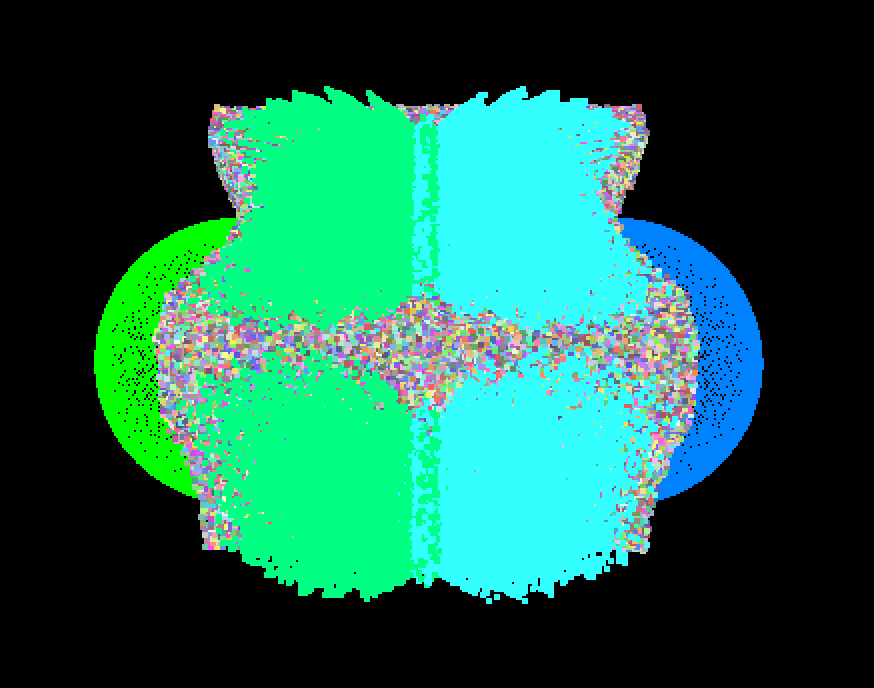
\includegraphics[width=14cm]{pic4}
		\caption{Phase 4}
	\end{figure}

	\begin{figure}[H]
		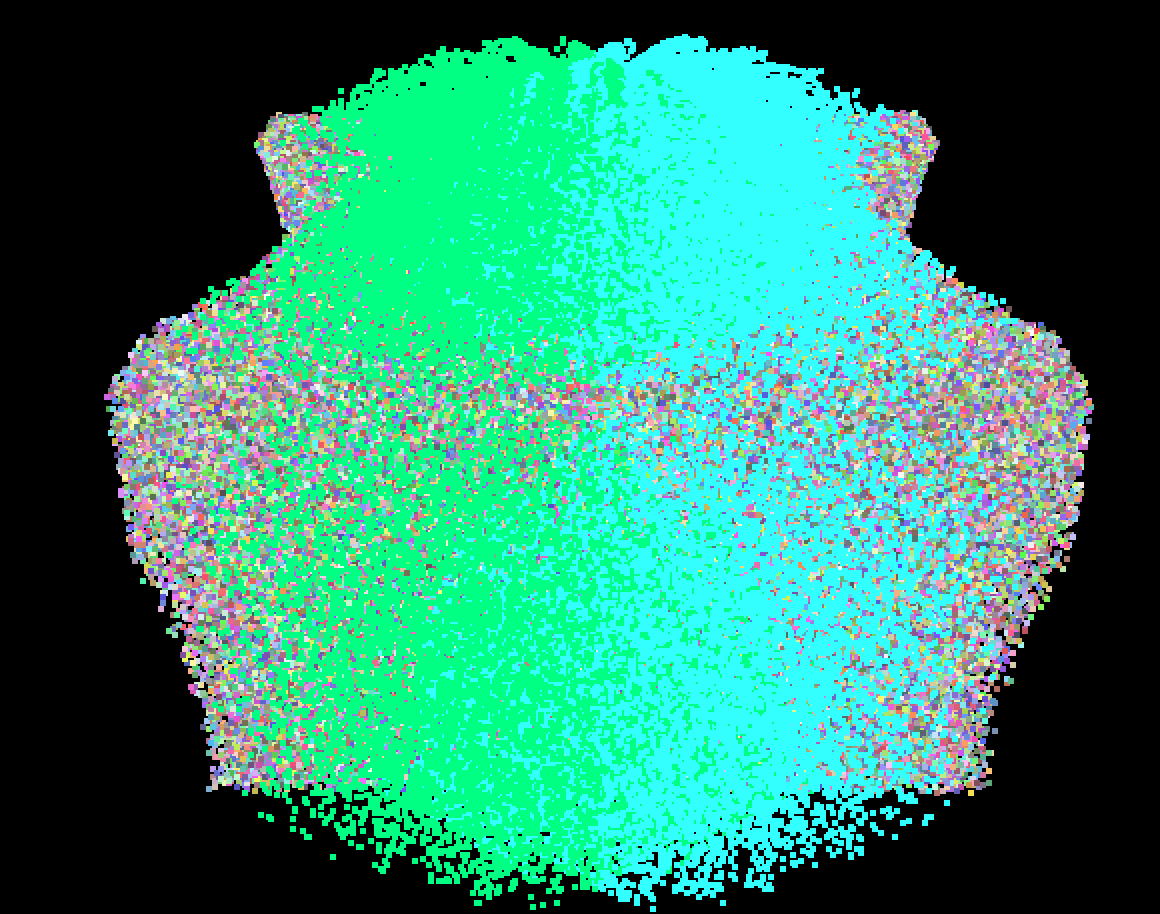
\includegraphics[width=16cm]{pic5}
		\centering
		\caption{Phase 5}
	\end{figure}
	
	
	



\section{Results Table}

	\begin{figure}[H]
		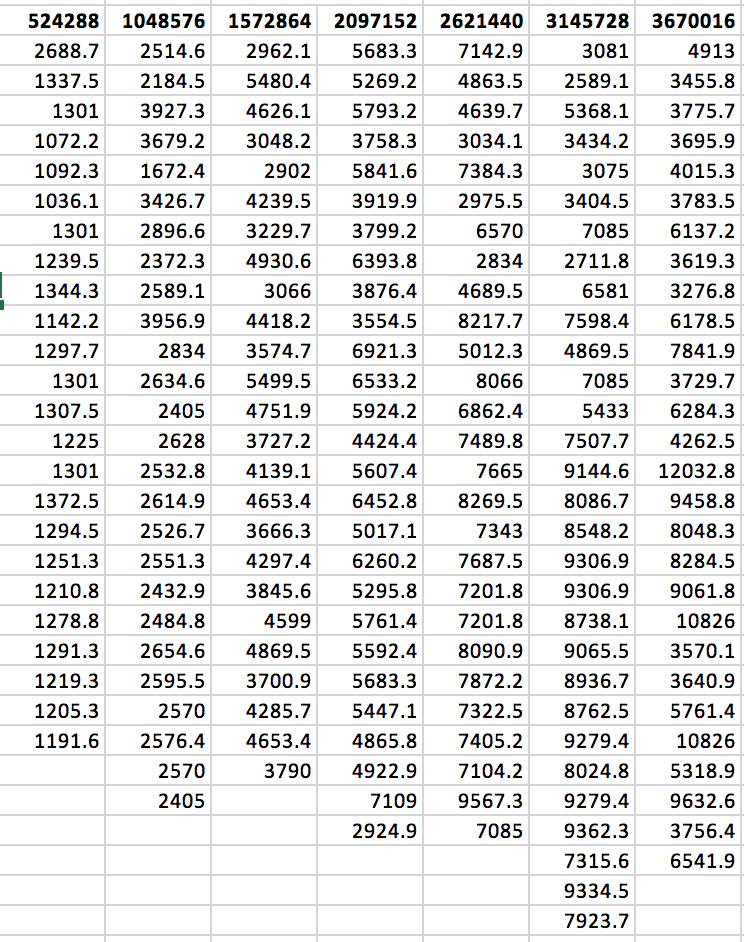
\includegraphics[width=16cm]{table}
		\centering
		\caption{A table of the OpenGL/OpenCL interoperability results. The bold first row is the total number of particles in that experiment, and the non-bolded numbers in its column are the \textit{megaParticles per second} values}
	\end{figure}





\section{Results Graph}
	\begin{figure}[H]
		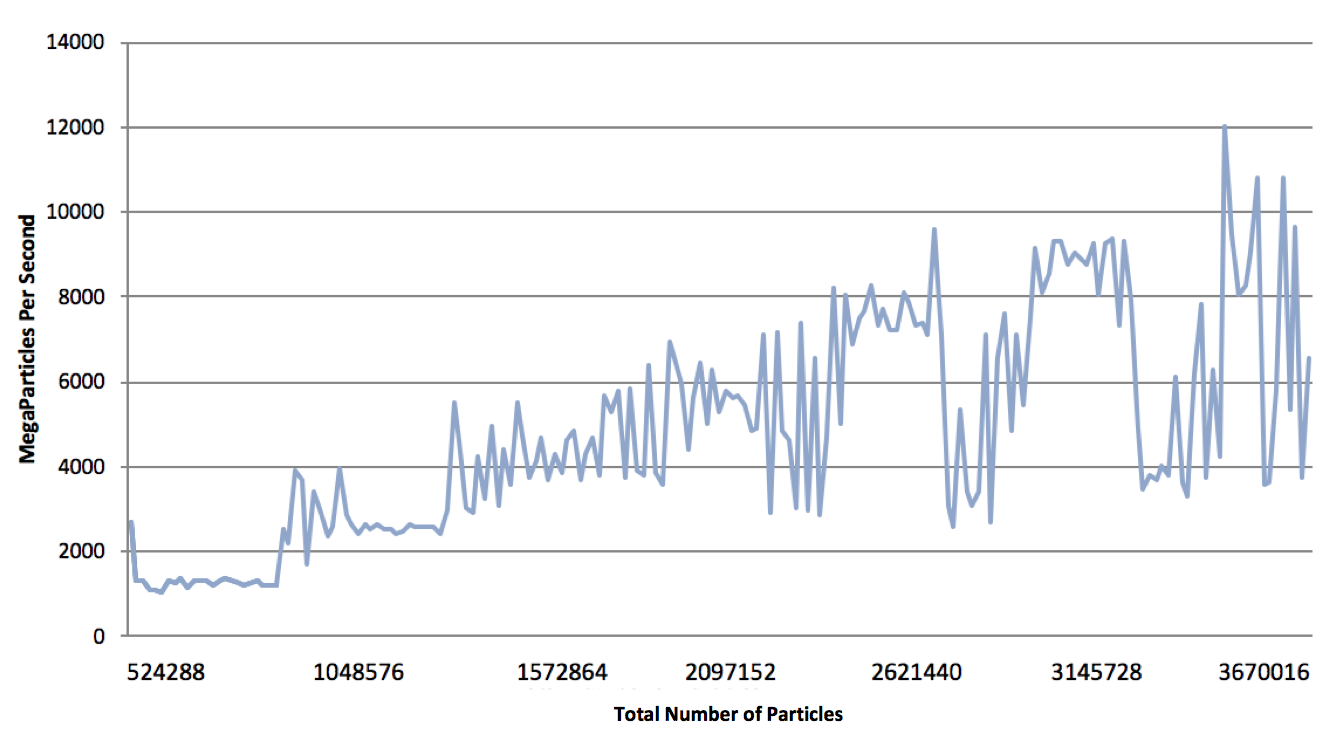
\includegraphics[width=16cm]{graph}
		\centering
		\caption{A graph of the \textit{MegaParticles Per Second} vs. \textit{Total Number of Particles}}
	\end{figure}


				

			
	





	


\section{What patterns are you seeing in the performance curve?}
	The single curve looks like a three year snapshot of the stock market. It has frequent peaks and dips, but the overall trend is upwards as the total number of particles increases. 











\section{Why do you think the patterns look this way?}
	As we have discussed, GPU's are built for particle systems. So, this is a perfect scenario where the GPU can show off its power. I think the overall trend is upwards as the total number of particles increases, because the GPU can still hammer out more particles, i.e. I havn't reached the GPU's max performance.
	As for the dips in performance, those are due to taking performance samples every 50 times the \textit{Display()} function is entered instead of each iteration. The performance metric could have been low in the 50th time to the function. I calculated the averages  and got \dots
	
	\begin{tabular}{c|c}
		\hline 
		\textbf{Total Number of Particles} & \textbf{Average MegaParticles per Second} \\ \hline	
		524288 & 1304 \\ \hline
		1048676 & 3905 \\ \hline
		1572864& 8179 \\ \hline
		2097152& 12856 \\ \hline
		2621440& 19508 \\ \hline
		3145728& 24565 \\ \hline
		3670016& 32453 \\ \hline
	\end{tabular}

	As one can see by looking at the averages, the performance indeed increases steadily with the total number of particles.









\section{What does that mean for the proper use of GPU parallel computing?}
	This means for the proper use of GPU parallel computing, or, at least to maximize its performance, one should break the problem down into "particle like" sizes. The user should also do some testing and output the performance to find how many particles they can hand off to the GPU to maximize its performance. 


\end{document}